\clearpage

\section{Alice QKD}

\maketitle
This block is the main processor for Alice. 

AliceQKD is a superblock intended work as Alice's main processor. It performs a 
series of functions, including classical channel communication with Bob and 
data processing for basis reconciliation, error correction and privacy 
amplification.

\subsection*{Input Parameters}

%\begin{itemize}

%\end{itemize}

\subsection*{Methods}
%AliceQKD (vector <Signal*> \&inputSignals, vector <Signal*> \&outputSignals) : 
%Block(inputSignals, outputSignals) \{\};
%
%void initialize(void);
%
%bool runBlock(void);
%
%void setRateOfPhotons(double RPhotons) \{ RateOfPhotons = RPhotons; \};
%double const getRateOfPhotons(void) \{ return RateOfPhotons; \};
%
%void setStringPhotonsLength(int pLength) \{ StringPhotonsLength = pLength; \};
%int const getStringPhotonsLength(void) \{ return StringPhotonsLength; \};
%

\subsection*{Functional description}

\begin{figure}[H]
	\centering
	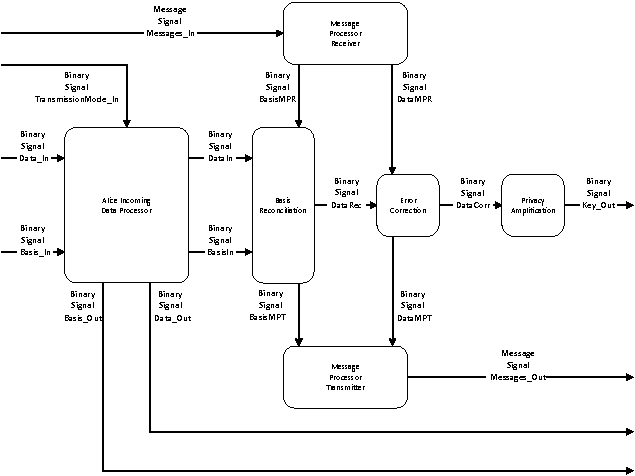
\includegraphics{./lib/alice_qkd2/figures/AliceQKD_blockDiagram.pdf}
\end{figure}

AliceQKD is a superblock intended to do classical channel communication and 
data processing  as required by the BB84 protocol. This superblock requires 
four different inputs:

\begin{itemize}
	\item Messages from Bob, which are used to coordinate the required data 
	processing for key extraction;
	\item A binary signal to be used for the transmitted key;
	\item A binary signal corresponding to the basis which will be used for 
	encoding the data.
	\item A binary signal controlling the transmission mode, enabling or 
	disabling transmission.
\end{itemize}

In addition, this block produces a total of five output signals:

\begin{itemize}
	\item	Messages intended to be read by Bob, used to coordinate the required 
	data processing for key extraction;
	\item A binary signals of the data, to be transmitted through the quantum 
	channel;
	\item A binary signal corresponding to the basis which will be used to 
	encoded the transmitted data;
	\item A binary signal with the generated key;
	\item A binary signal corresponding to the transmission control.
\end{itemize}


The process inside the superblock is as follows:

The incoming data and basis binary signals are provided as inputs to the 
\textit{AliceIncomingDataProcessor}, together with the 
\textit{transmissionMode} signal. 
The transmission mode controls the behaviour of the 
\textit{AliceIncomingDataProcessor}: it either enables it to continue working 
or tells it to stop reading the input data.
The data and basis read at the block are sent twice each to the output signals, 
keeping their sync. Each pair of basis and data has a different destination: 
one of the pair is directed to the superblock outputs, in order to transmit the 
data and control the basis for the transmission; and the other pair is sent to 
the \textit{BasisReconciliation} block.

The \textit{BasisReconciliation} block in AliceQKD is configured to responding
to Bobs messages, instead of sending them first. Therefore, it now waits for a 
signal from the 
\textit{MessageProcessorReceiver}. When Bob has enough samples, he should send 
a message containing the basis he used to measure the received data. This 
message is received, identified by its type \texttt{BasisReconciliation1}, and 
interpreted at the \textit{MessageProcessorReceiver}. 
When a message of the correct type arrives, this block sends a signal to the 
\textit{BasisReconcilliation} block, containing the list of basis Bob used to 
measure the data on his side. The \textit{BasisReconciliation} block then 
compares the basis received from Bob with the ones that Alice used, and based 
on this is outputs two signals:

\begin{itemize}
	\item A binary evaluation of which basis used 
	by Bob are correct. This is sent to the \textit{MessageProcessorTransmitter}, 
	so that a message can be sent to Bob for him to know which basis were correct.
	\item A binary signal containing the data sent when those basis were used. 
	This is the data that Bob should have measured correctly. This signal is sent 
	to the \textit{ErrorCorrection} block.
\end{itemize} 

The \textit{ErrorCorrection} block will be responsible for correcting any 
errors that occurred during transmission. Similarly to the 
\textit{BasisReconciliation} block, it is configured to act in response to Bobs 
messages. As such, it waits for data from the 
\textit{MessageProcessorReceiver}, and outputs a response to the 
\textit{MessageProcessorTransmitter}. It also outputs a copy of the 
signal from basis reconciliation, after it has been used for error correction. 
This is will be the transmitted key, free from errors.

%There is also an auxiliary binary signal which goes from block's output to its 
%input. The purpose of this signal is to aid in

When the \textit{MessageProcessorReceiver} receives a message with the type 
\texttt{ErrorCorrection1}, it starts the Cascade error correction process.
That message contains the necessary information used in the Cascade process. 
The explanation of the whole error correction process is somewhat long and not 
required to understand how the AliceQKD block works. Therefore, further details 
can be found in the \textit{ErrorCorrection} block's documentation.

After each set of bits is corrected, the data is output to the 
\textit{PrivacyAmplification} block, which does the necessary transformation to 
ensure the information that any attacker might have gained (Eve) is nullified.

The end result, and final output of the superblock, is a secure key 
shared known only to Alice and Bob.

As mentioned before, this whole process is controlled by the 
\textit{transmissionMode} signal.

\subsection*{Input Signals}
\paragraph*{Number}: 3
\paragraph*{Type}: Binary, Real Continuous Time and Messages signals.

\subsection*{Output Signals}
\paragraph*{Number}: 4
\paragraph*{Type}: Binary, Real Discrete Time and Messages signals.

\subsection*{Examples}


\subsection*{Sugestions for future improvement}












%\clearpage
%
%\section{Alice QKD}
%
%\maketitle
%This block is the processor for Alice does all tasks that she needs. This 
%block accepts binary, messages, and real continuous time signals. It produces 
%messages, binary and real discrete time signals.
%
%
%\subsection*{Input Parameters}
%
%	\begin{itemize}
%		\item double RateOfPhotons\{1e3\}
%	
%		\item int StringPhotonsLength\{ 12 \}
%	\end{itemize}
%
%\subsection*{Methods}
%    AliceQKD (vector <Signal*> \&inputSignals, vector <Signal*> 
%\&outputSignals) : Block(inputSignals, outputSignals) \{\};
%
%	void initialize(void);
%
%	bool runBlock(void);
%
%	void setRateOfPhotons(double RPhotons) \{ RateOfPhotons = RPhotons; \};
%	double const getRateOfPhotons(void) \{ return RateOfPhotons; \};
%
%	void setStringPhotonsLength(int pLength) \{ StringPhotonsLength = pLength; \};
%	int const getStringPhotonsLength(void) \{ return StringPhotonsLength; \};
%
%
%\subsection*{Functional description}
%
%This block receives a sequence of binary numbers (1's or 0's) and a clock 
%signal which will set the rate of the signals produced to generate single 
%polarized photons. The real discrete time signal \textbf{SA\_1} is generated 
%based on the clock signal and the real discrete time signal \textbf{SA\_2} is 
%generated based on the random sequence of bits received through the signal 
%\textbf{NUM\_A}. This last sequence is analysed by the polarizer in pairs of 
%bits in which each pair has a bit for basis choice and other for direction 
%choice.
%
%This block also produces classical messages signals to send to Bob as well as 
%binary messages to the mutual information block with information about the 
%photons it sent.
%
%\subsection*{Input Signals}
%\paragraph*{Number}: 3
%\paragraph*{Type}: Binary, Real Continuous Time and Messages signals.
%
%\subsection*{Output Signals}
%\paragraph*{Number}: 3
%\paragraph*{Type}: Binary, Real Discrete Time and Messages signals.
%
%\subsection*{Examples}
%
%
%\subsection*{Sugestions for future improvement}
%
%
%
